\documentclass[a4paper,12pt]{article}
% Package to make citations superscrit with brackets
\usepackage[super,square]{natbib}
% Package to change margin size
\usepackage{anysize}
\usepackage{amsmath}
\marginsize{2cm}{2cm}{1cm}{2cm}
% Package to make headers
\usepackage{fancyhdr}
\usepackage{circuitikz}
\renewcommand{\headrulewidth}{0pt}
\usepackage{soul}
\usepackage[section]{placeins}
% Colors for the references links
\usepackage[dvipsnames]{xcolor}
% Package to link references
\usepackage{hyperref}
\usepackage{graphicx}
\hypersetup{
 colorlinks=true,
  linkcolor=black,
  citecolor=CadetBlue,  
  filecolor=CadetBlue,      
  urlcolor=CadetBlue,
}
% Package for lorem ipsum
\usepackage{lipsum}
% Package for multicolumn
\usepackage{multicol}
% Package for removing paragraph identations
\usepackage{parskip}
\setlength\columnsep{18pt}
% Sets bastract
\renewenvironment{abstract}
{\par\noindent\textbf{\abstractname}\ \ignorespaces \\}
{\par\noindent\medskip}




\begin{document}
% Makes header
\pagestyle{fancy}
\thispagestyle{empty}
\fancyhead[R]{\textit{EE1200}}
\fancyhead[L]{}
% Makes footnotes with an asterisk
\renewcommand*{\thefootnote}{\fnsymbol{footnote}}
\begin{center}
  \Large{\textbf{Experiment 03}}
  \vspace{0.4cm}
  \normalsize
  \\ Aditya Tripathy - ee24btech11001, Durgi Swaraj Sharma - ee24btech11018\\
  \medskip
  \normalsize
\end{center}
{\color{gray}\hrule}
\vspace{0.4cm}
\begin{abstract}
  In Experiment-03, we studied the amplitude and phase responses of 1-stage, 2-stage, 3-stage RC low pass filters to a sinusoidal wave input over a range of frequencies.
\end{abstract}
{\color{gray}\hrule}
\medskip
\section{Objective}
To study, measure, and plot the frequency-amplitude and frequency-phase response of 1-stage, 2-stage, 3-stage RC low pass circuits to a sinusoidal wave input. 
\section{Apparatus}
\begin{itemize}
  \item Oscilloscope
  \item Function generator
  \item Connecting wires and probes
  \item Unpolarised capacitors
  \item Resistors
\end{itemize}
\section{Theory}

We derive the transfer functions for cascaded 1-stage, 2-stage, 3-stage RC low-pass filters, assuming that all resistors and capacitors have the same values:  
\[
R_1 = R_2 = R_3 = R, \quad C_1 = C_2 = C_3 = C.
\]
The output is measured at the last capacitor in the chain.

\subsection{1-stage RC Network}

For a single-stage RC low-pass filter, the circuit consists of a resistor \( R \) in series with a capacitor \( C \), with the output taken across the capacitor. The impedance of the capacitor is:
\[
Z_C = \frac{1}{j\omega C}.
\]
Applying the voltage divider rule, the transfer function is:
\[
H_1(j\omega) = \frac{Z_C}{R + Z_C} = \frac{\frac{1}{j\omega C}}{R + \frac{1}{j\omega C}}.
\]
Multiplying numerator and denominator by \( j\omega C \), we obtain:
\[
H_1(j\omega) = \frac{1}{1 + j\omega RC}.
\]

\subsection{2-stage RC Network}

For a two-stage RC network, the first RC stage loads the second, so the second stage must account for the finite impedance of the first stage. The first stage's output voltage is:
\[
V_1 = H_1(j\omega) V_{\text{in}} = \frac{V_{\text{in}}}{1 + j\omega RC}.
\]
The second stage is another RC circuit with input \( V_1 \), where the equivalent resistance looking back into the first stage is modified. The voltage divider for the second stage is:
\[
H_2(j\omega) = \frac{Z_C}{R + Z_C + \frac{R}{1 + j\omega RC}}.
\]
Substituting \( Z_C = \frac{1}{j\omega C} \) and simplifying, we obtain:
\[
H_2(j\omega) = \frac{1}{1 + 3j\omega RC - \omega^2 R^2C^2}.
\]

\subsection{3-stage RC Network}

For a three-stage RC network, the output from the second stage serves as the input to the third stage. The second-stage voltage is:
\[
V_2 = H_2(j\omega) V_{\text{in}}.
\]
Applying the voltage divider rule for the third stage while considering the impedance of the preceding stages, the transfer function becomes:
\[
H_3(j\omega) = \frac{1}{1 + 6j\omega RC - 5\omega^2 R^2C^2 - j\omega^3 R^3C^3}.
\]

\begin{figure}
  \centering
  \resizebox{0.18\textwidth}{!}{%
    \begin{circuitikz}
      \tikzstyle{every node}=[font=\LARGE]
      \draw (8.25,16.5) to[european resistor,l={ \LARGE $R_1$}] (8.25,14);
      \draw (8.25,16.5) to[short] (5.5,16.5);
      \draw (5.5,16.5) to[sinusoidal voltage source, sources/symbol/rotate=auto] (5.5,8.25);
      \draw (7,8.25) to[short] (5.5,8.25);
      \draw (8.25,14) to[C,l={ \LARGE $C_1$}] (8.25,8.25);
      \draw (7,8.25) to[short] (8.25,8.25);
    \end{circuitikz}
    }
    \caption{1-stage RC Low pass filter}
    \resizebox{0.28\textwidth}{!}{%
      \begin{circuitikz}
        \tikzstyle{every node}=[font=\LARGE]
        \draw (8.25,16.5) to[european resistor,l={ \LARGE $R_1$}] (8.25,14);
        \draw (8.25,13.75) to[short] (9.75,13.75);
        \draw (9.75,13.75) to[european resistor,l={ \LARGE $R_2$}] (9.75,11.5);
        \draw (8.25,16.5) to[short] (5.5,16.5);
        \draw (5.5,16.5) to[sinusoidal voltage source, sources/symbol/rotate=auto] (5.5,8.25);
        \draw (7,8.25) to[short] (5.5,8.25);
        \draw (8.25,14) to[C,l={ \LARGE $C_1$}] (8.25,8.25);
        \draw (9.75,11.5) to[C,l={ \LARGE $C_2$}] (9.75,8.25);
        \draw (9.75,8.25) to[short] (6.75,8.25);
      \end{circuitikz}
      }
      \caption{2-stage RC Low pass filter}
      \resizebox{0.29\textwidth}{!}{%
        \begin{circuitikz}
          \tikzstyle{every node}=[font=\LARGE]
          \draw (8.25,16.5) to[european resistor,l={ \LARGE $R_1$}] (8.25,14);
          \draw (8.25,13.75) to[short] (9.75,13.75);
          \draw (9.75,13.75) to[european resistor,l={ \LARGE $R_2$}] (9.75,11.5);
          \draw (9.75,11.75) to[short] (11.25,11.75);
          \draw (11.25,11.75) to[european resistor,l={ \LARGE $R_3$}] (11.25,9.75);
          \draw (11.25,9.75) to[C,l={ \LARGE $C_3$}] (11.25,8.25);
          \draw (11.25,8.25) to[short] (7,8.25);
          \draw (8.25,16.5) to[short] (5.5,16.5);
          \draw (5.5,16.5) to[sinusoidal voltage source, sources/symbol/rotate=auto] (5.5,8.25);
          \draw (7,8.25) to[short] (5.5,8.25);
          \draw (8.25,14) to[C,l={ \LARGE $C_1$}] (8.25,8.25);
          \draw (9.75,11.5) to[C,l={ \LARGE $C_2$}] (9.75,8.25);
        \end{circuitikz}
        }
	\caption{3-stage RC Low pass filter}
\end{figure}
\section{Procedure}
\begin{enumerate}
  \item Connections
    \begin{itemize}
      \item Connect the function generator to the resistor end of the series RC, and associated ground to the capacitor end.
      \item Connect the first channel of the oscilloscope to the resistor end where the voltage is same as that from the function generator, and the associated ground to the common ground.
      \item Connect the second channel of the oscilloscope in between R and C, and the associated ground to the common ground.
      \item Ensure scaling is set to 10X both on the probe wires and the oscilloscope.
    \end{itemize}
  \item Cascading
    \begin{itemize}
      \item To cascade our RC ciruit once, connect another series-RC parallel to capacitor. 
      \item Move the oscilloscope probes from measuring across the initial capacitor to measuring across the new capacitor. 
      \item To cascade once more, repeat the previous steps over the second capacitor. 
    \end{itemize}
  \item Device setup and main process
    \begin{itemize}
      \item Set the frequency on the function generator to the lowest possible value, and amplitude as $1$V. Ensure its output is a sine wave.
      \item Utilize the cursor functions in the oscilloscope, and set them on the cloest crests in the two waves. 
      \item Measure the $\delta X$ value from the cursors, which gives you the phase difference when multiplied by the frequency. Measure the peak voltages, which will give you amplitude ratio. 
      \item Increase the frequency and repeat the process, until you reach the highest possible frequency on the function generator. 
    \end{itemize}
  \item Plotting
    \begin{itemize}
      \item On two graph sheets, use a logarithmic scale for both the axes. 
      \item On one of the sheets, plot the log of ratio of peak voltages along the vertical across the log of frequency they were obtained at along the horizontal. 
      \item On the other graph sheet, in a similar manner, plot the log of phase difference over the vertical instead. 
    \end{itemize}
  \item Repeat the main process and plotting for the 2-stage and 3-stage circuits.
\end{enumerate}
\section{Plotting and Justification}
We will be using Python along with Matplotlib and Numpy libraries to verify our experiment's results. The following are manual and verification plots of the frequency-amplitude and frequency-phase responses of 1-stage, 2-stage, and 3-stage RC circuit to the input sine wave. Please note that the second hand-plotted graph in each section is a plot between the phase and $log(\omega)$
\subsection{1-stage RC filter}
\begin{figure}[!ht]
\centering
  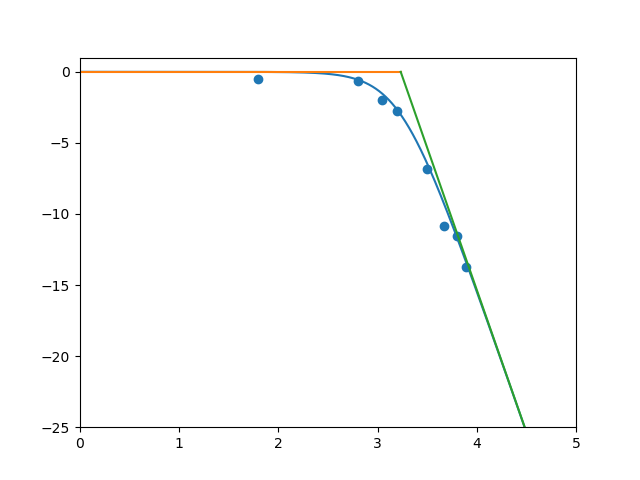
\includegraphics[width=0.4\columnwidth]{/home/gvt1/Work/ECLab2025/experiment03/files/fit.png}
  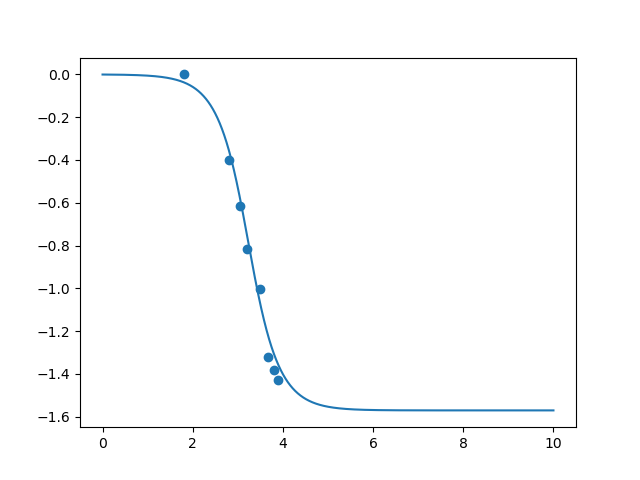
\includegraphics[width=0.4\columnwidth]{/home/gvt1/Work/ECLab2025/experiment03/files/phase_1.png}
  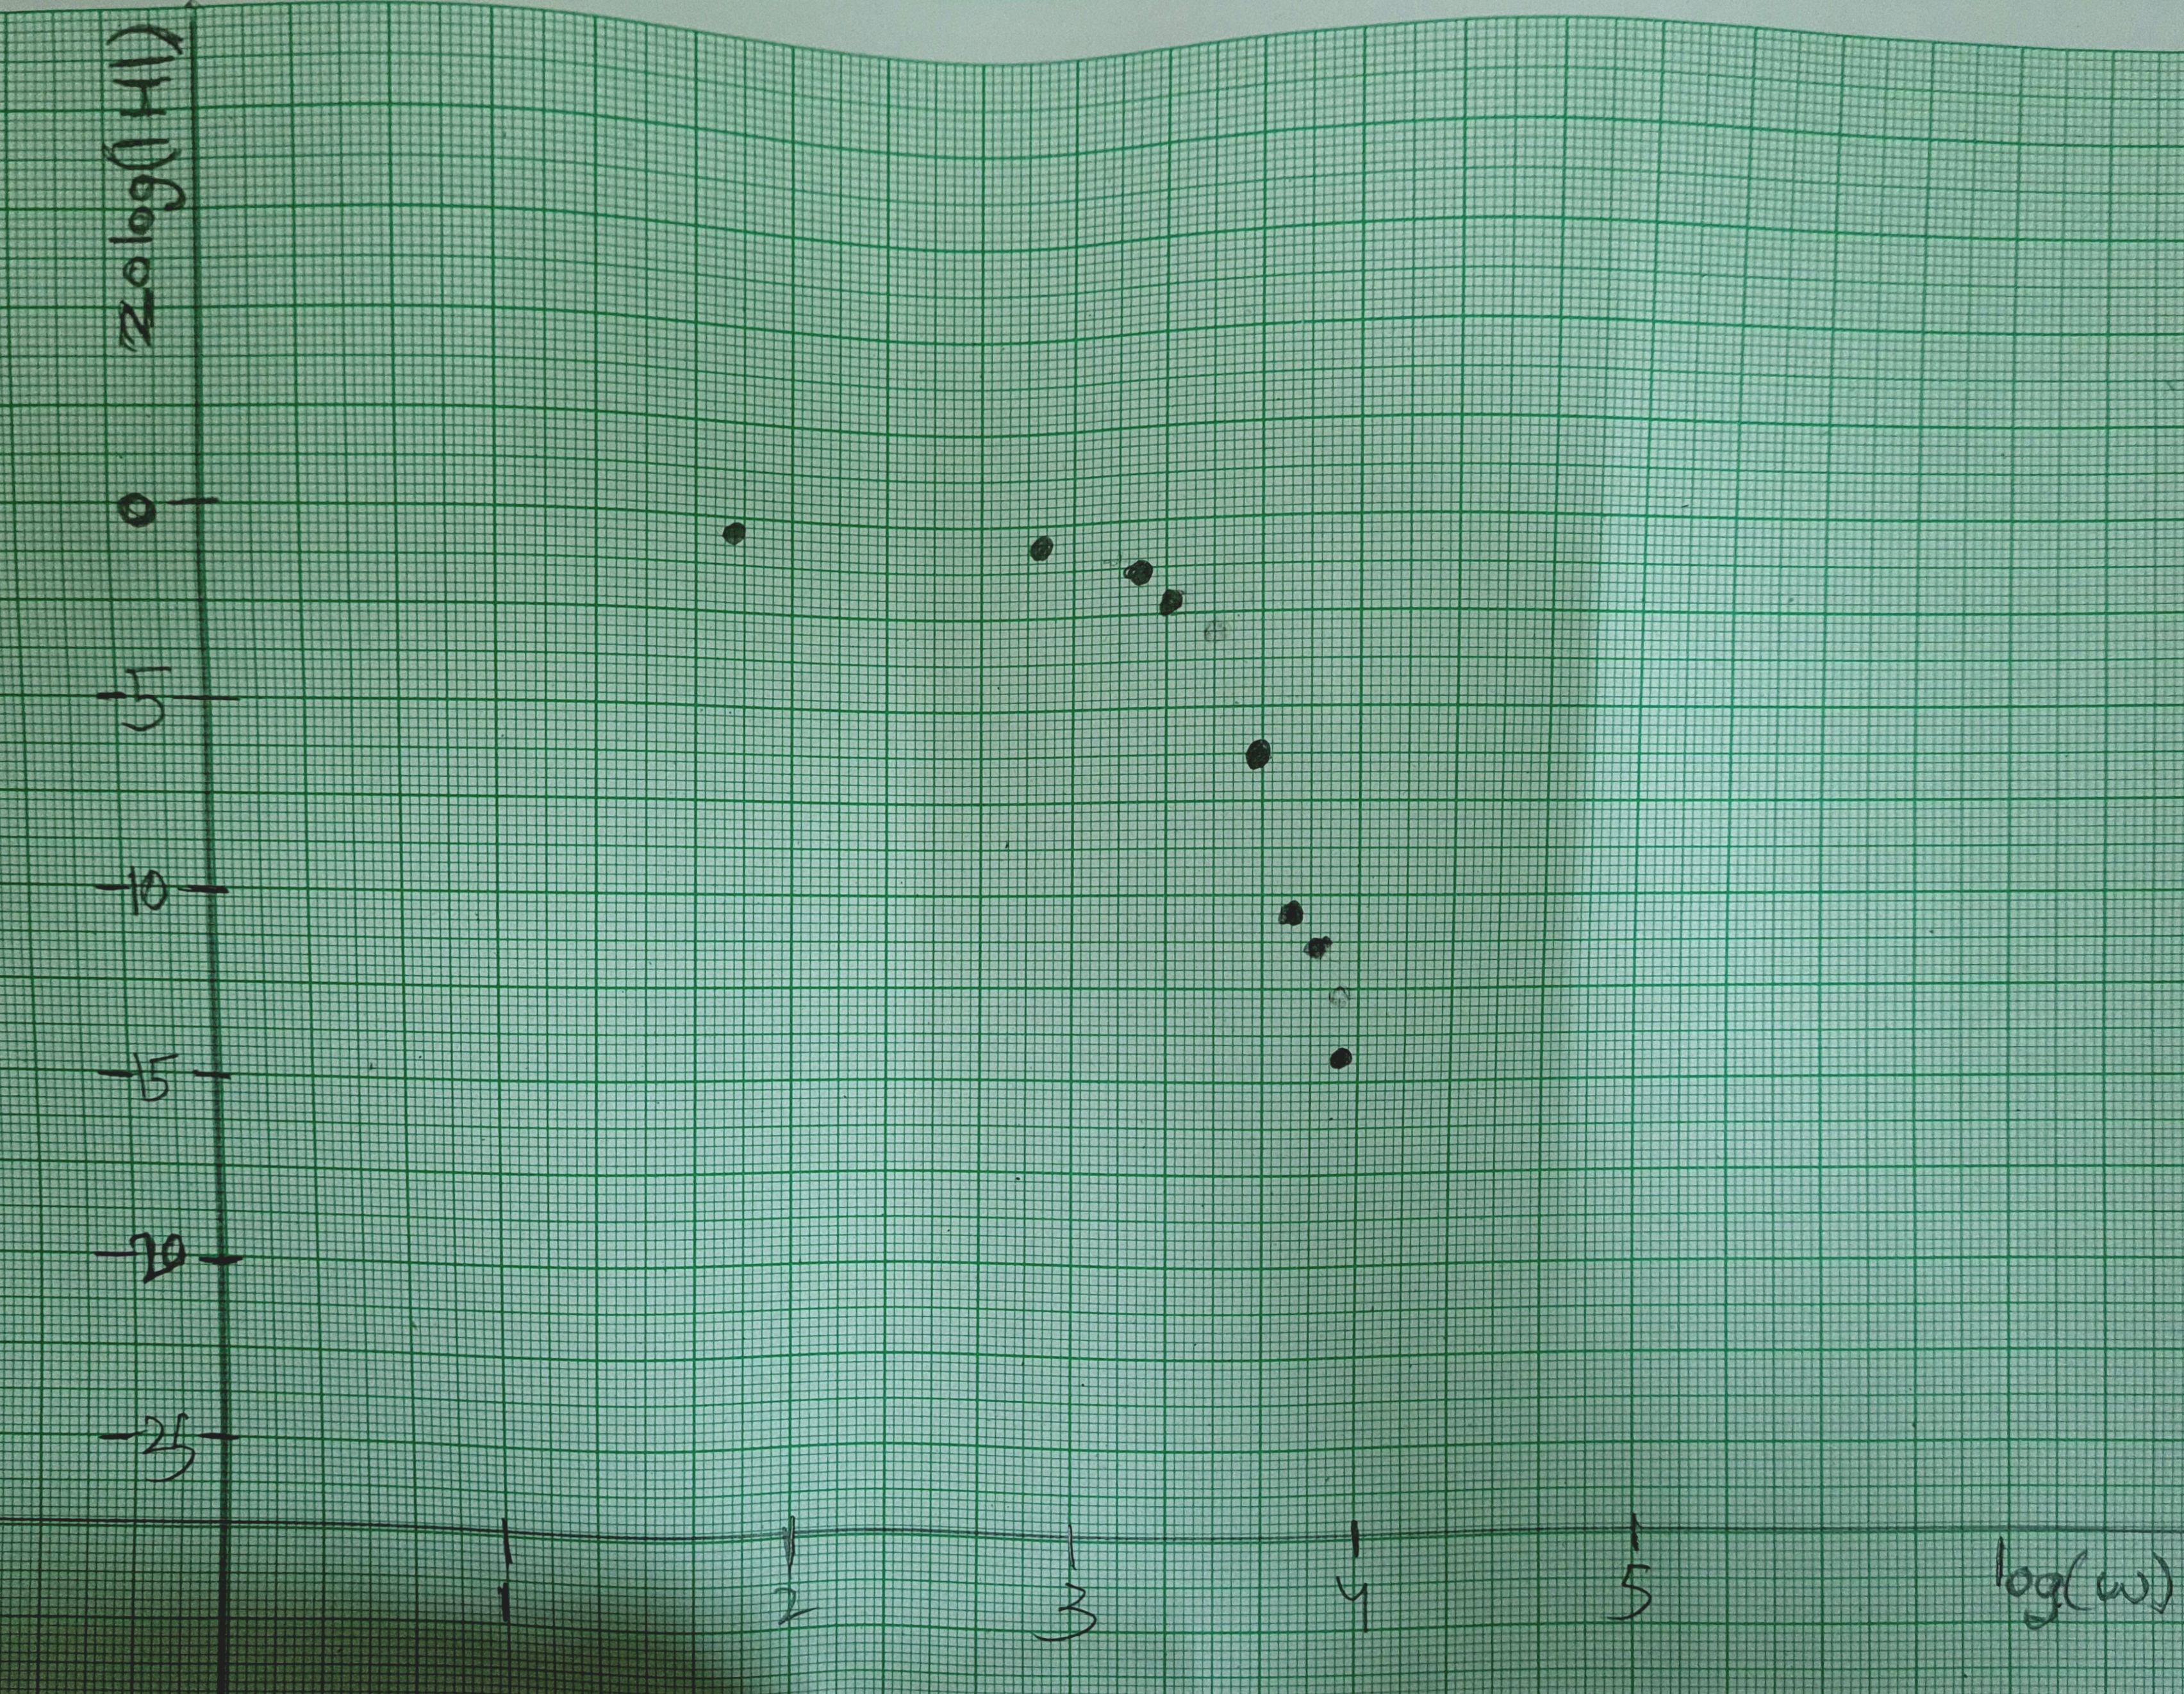
\includegraphics[width=0.7\columnwidth]{/home/gvt1/Work/ECLab2025/experiment03/files/GraphH1.jpg}
  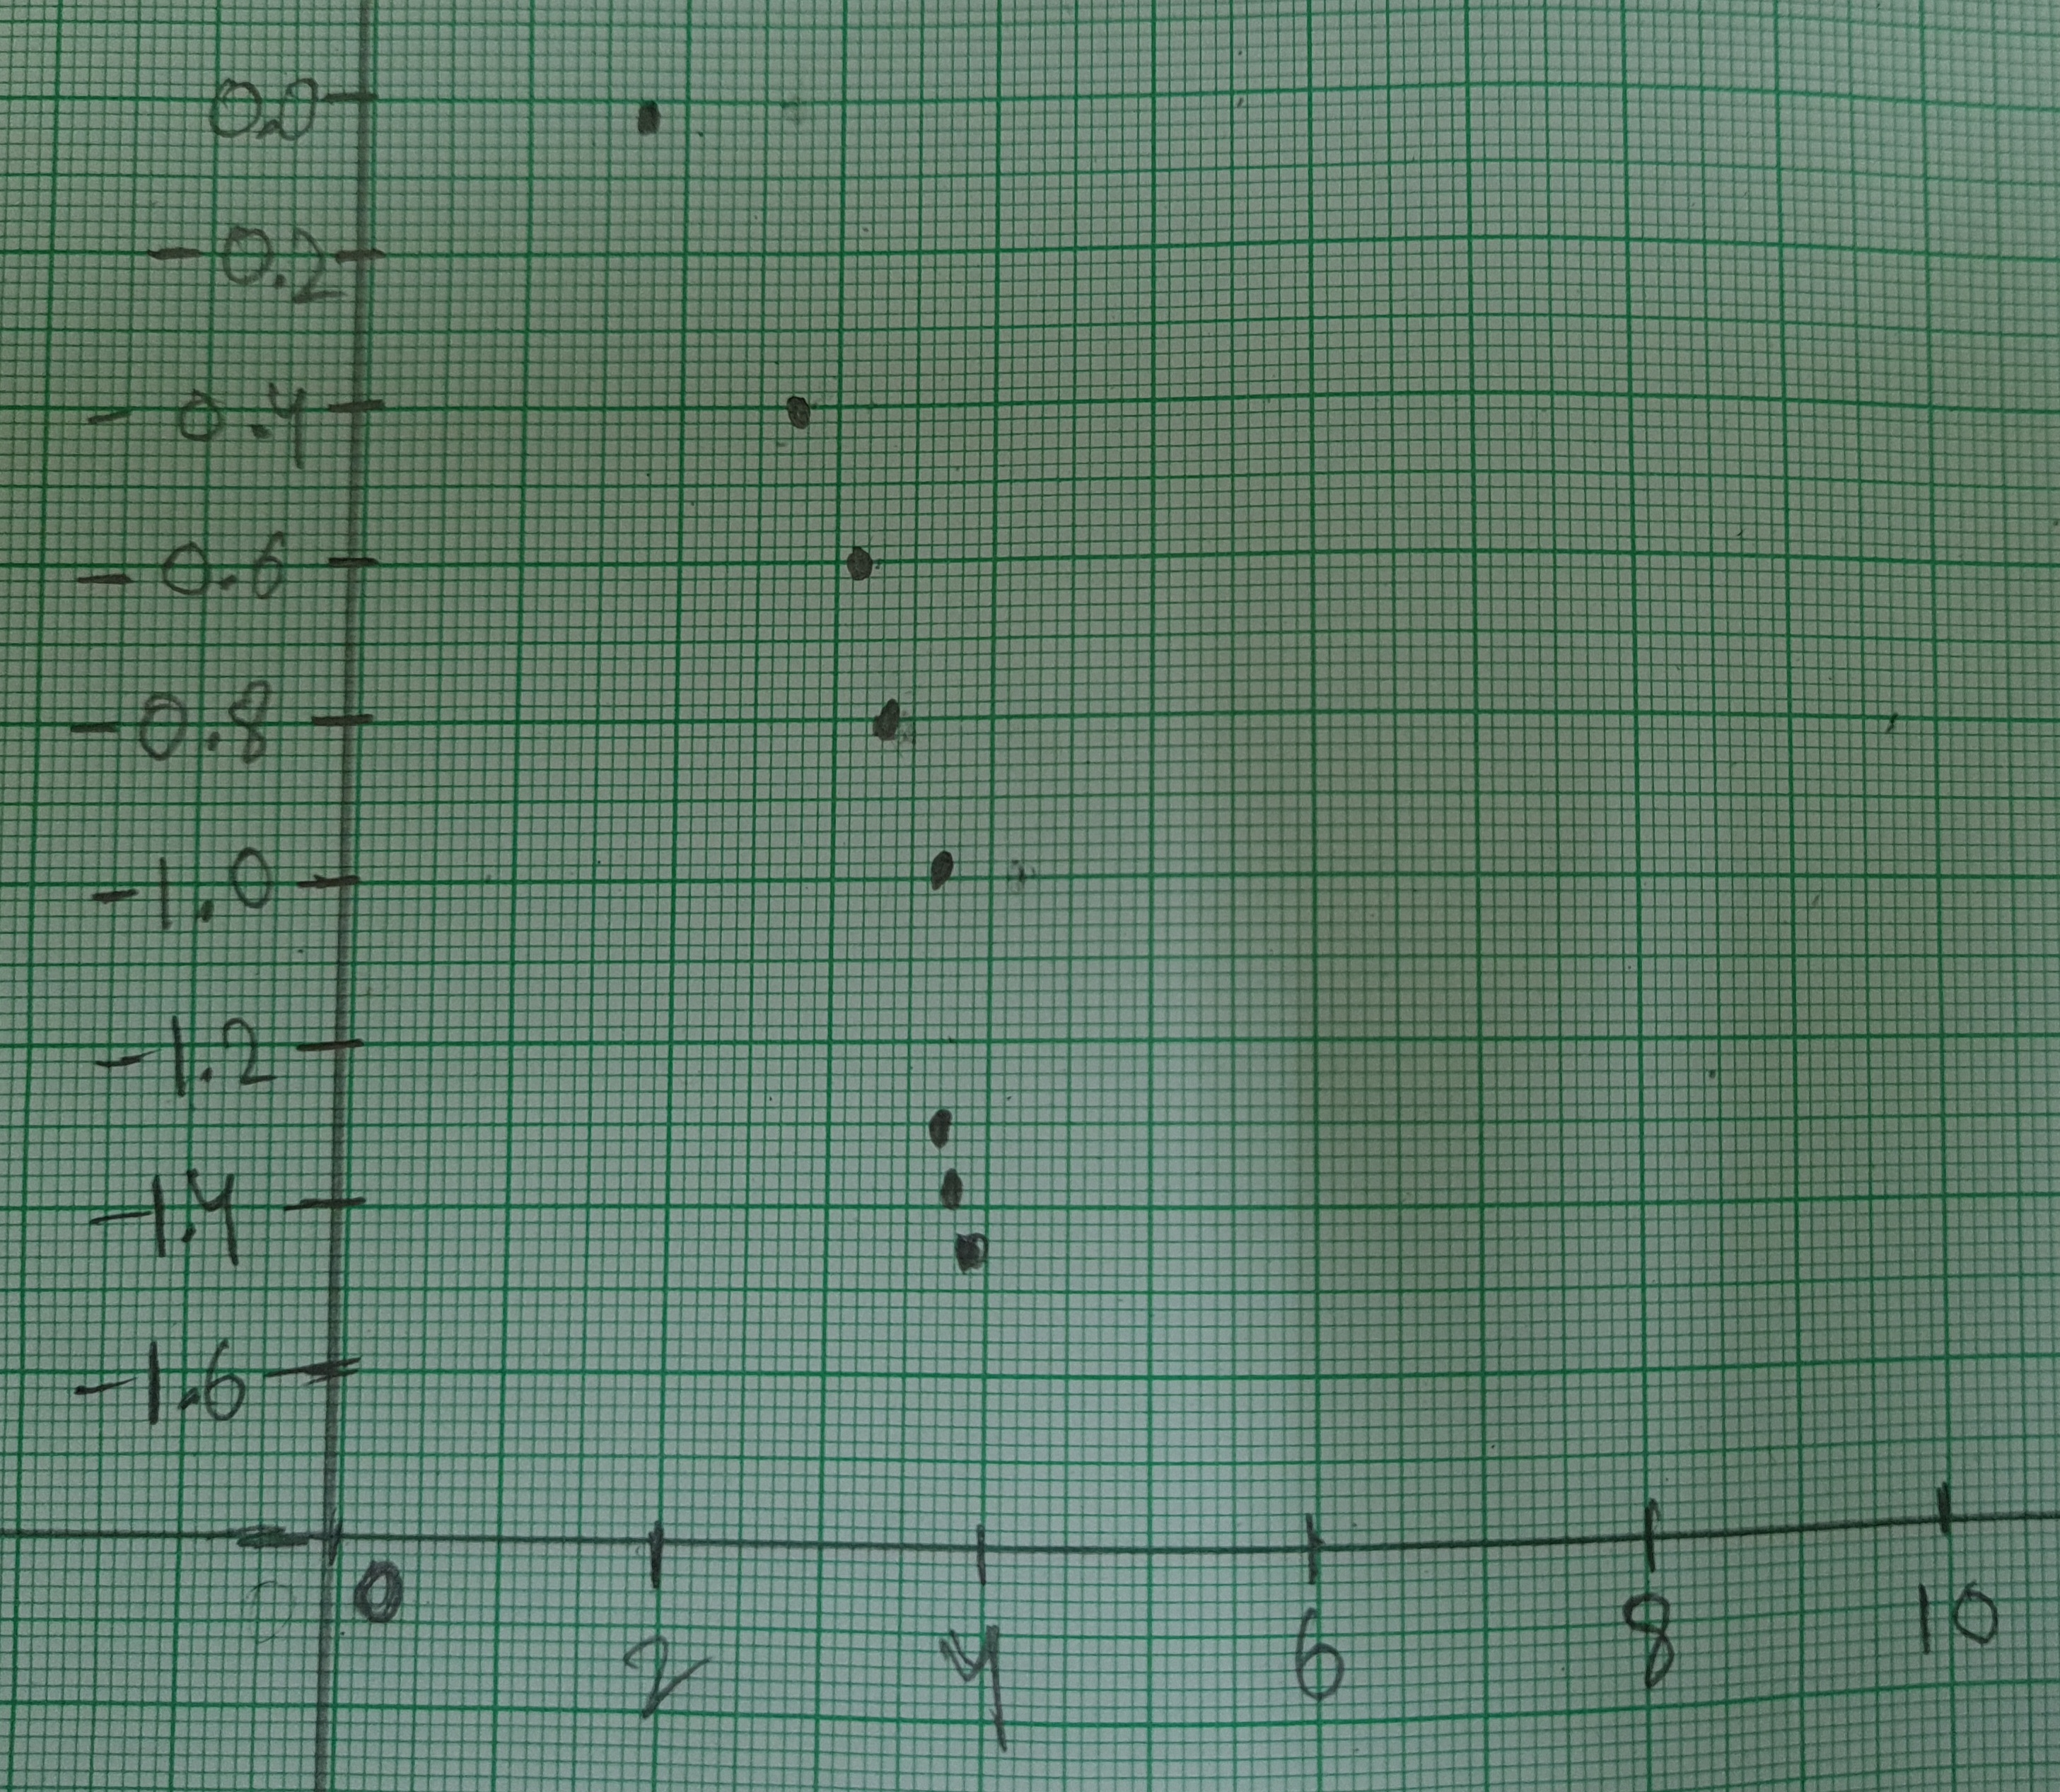
\includegraphics[width=0.4\columnwidth]{/home/gvt1/Work/ECLab2025/experiment03/files/GraphP1.jpg}
\end{figure}
\subsection{2-stage RC filter}
\begin{figure}[!ht]
\centering
  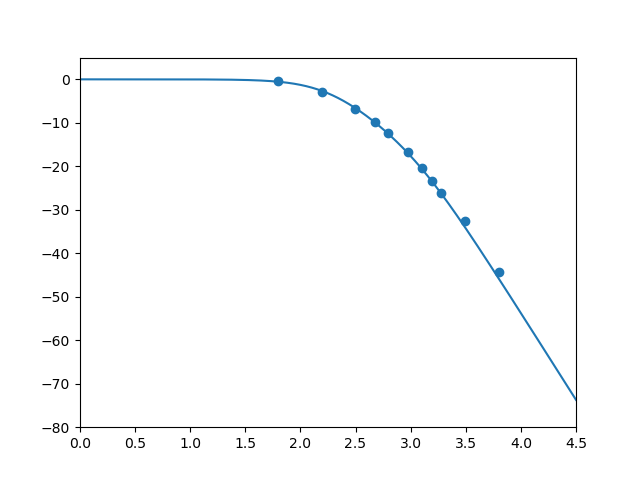
\includegraphics[width=0.4\columnwidth]{/home/gvt1/Work/ECLab2025/experiment03/files/fit_2.png}
  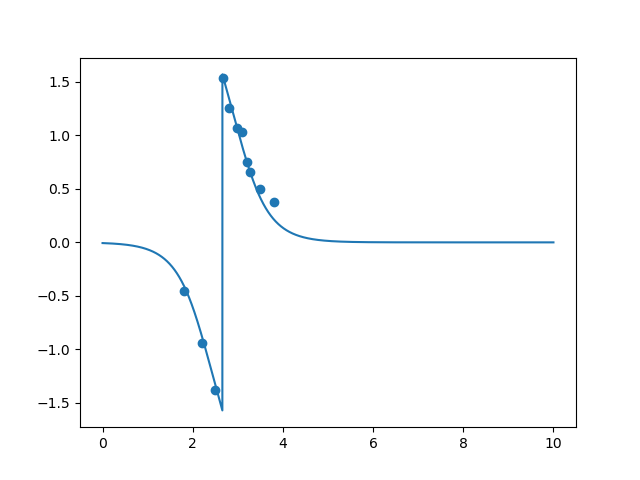
\includegraphics[width=0.4\columnwidth]{/home/gvt1/Work/ECLab2025/experiment03/files/phase_2.png}
  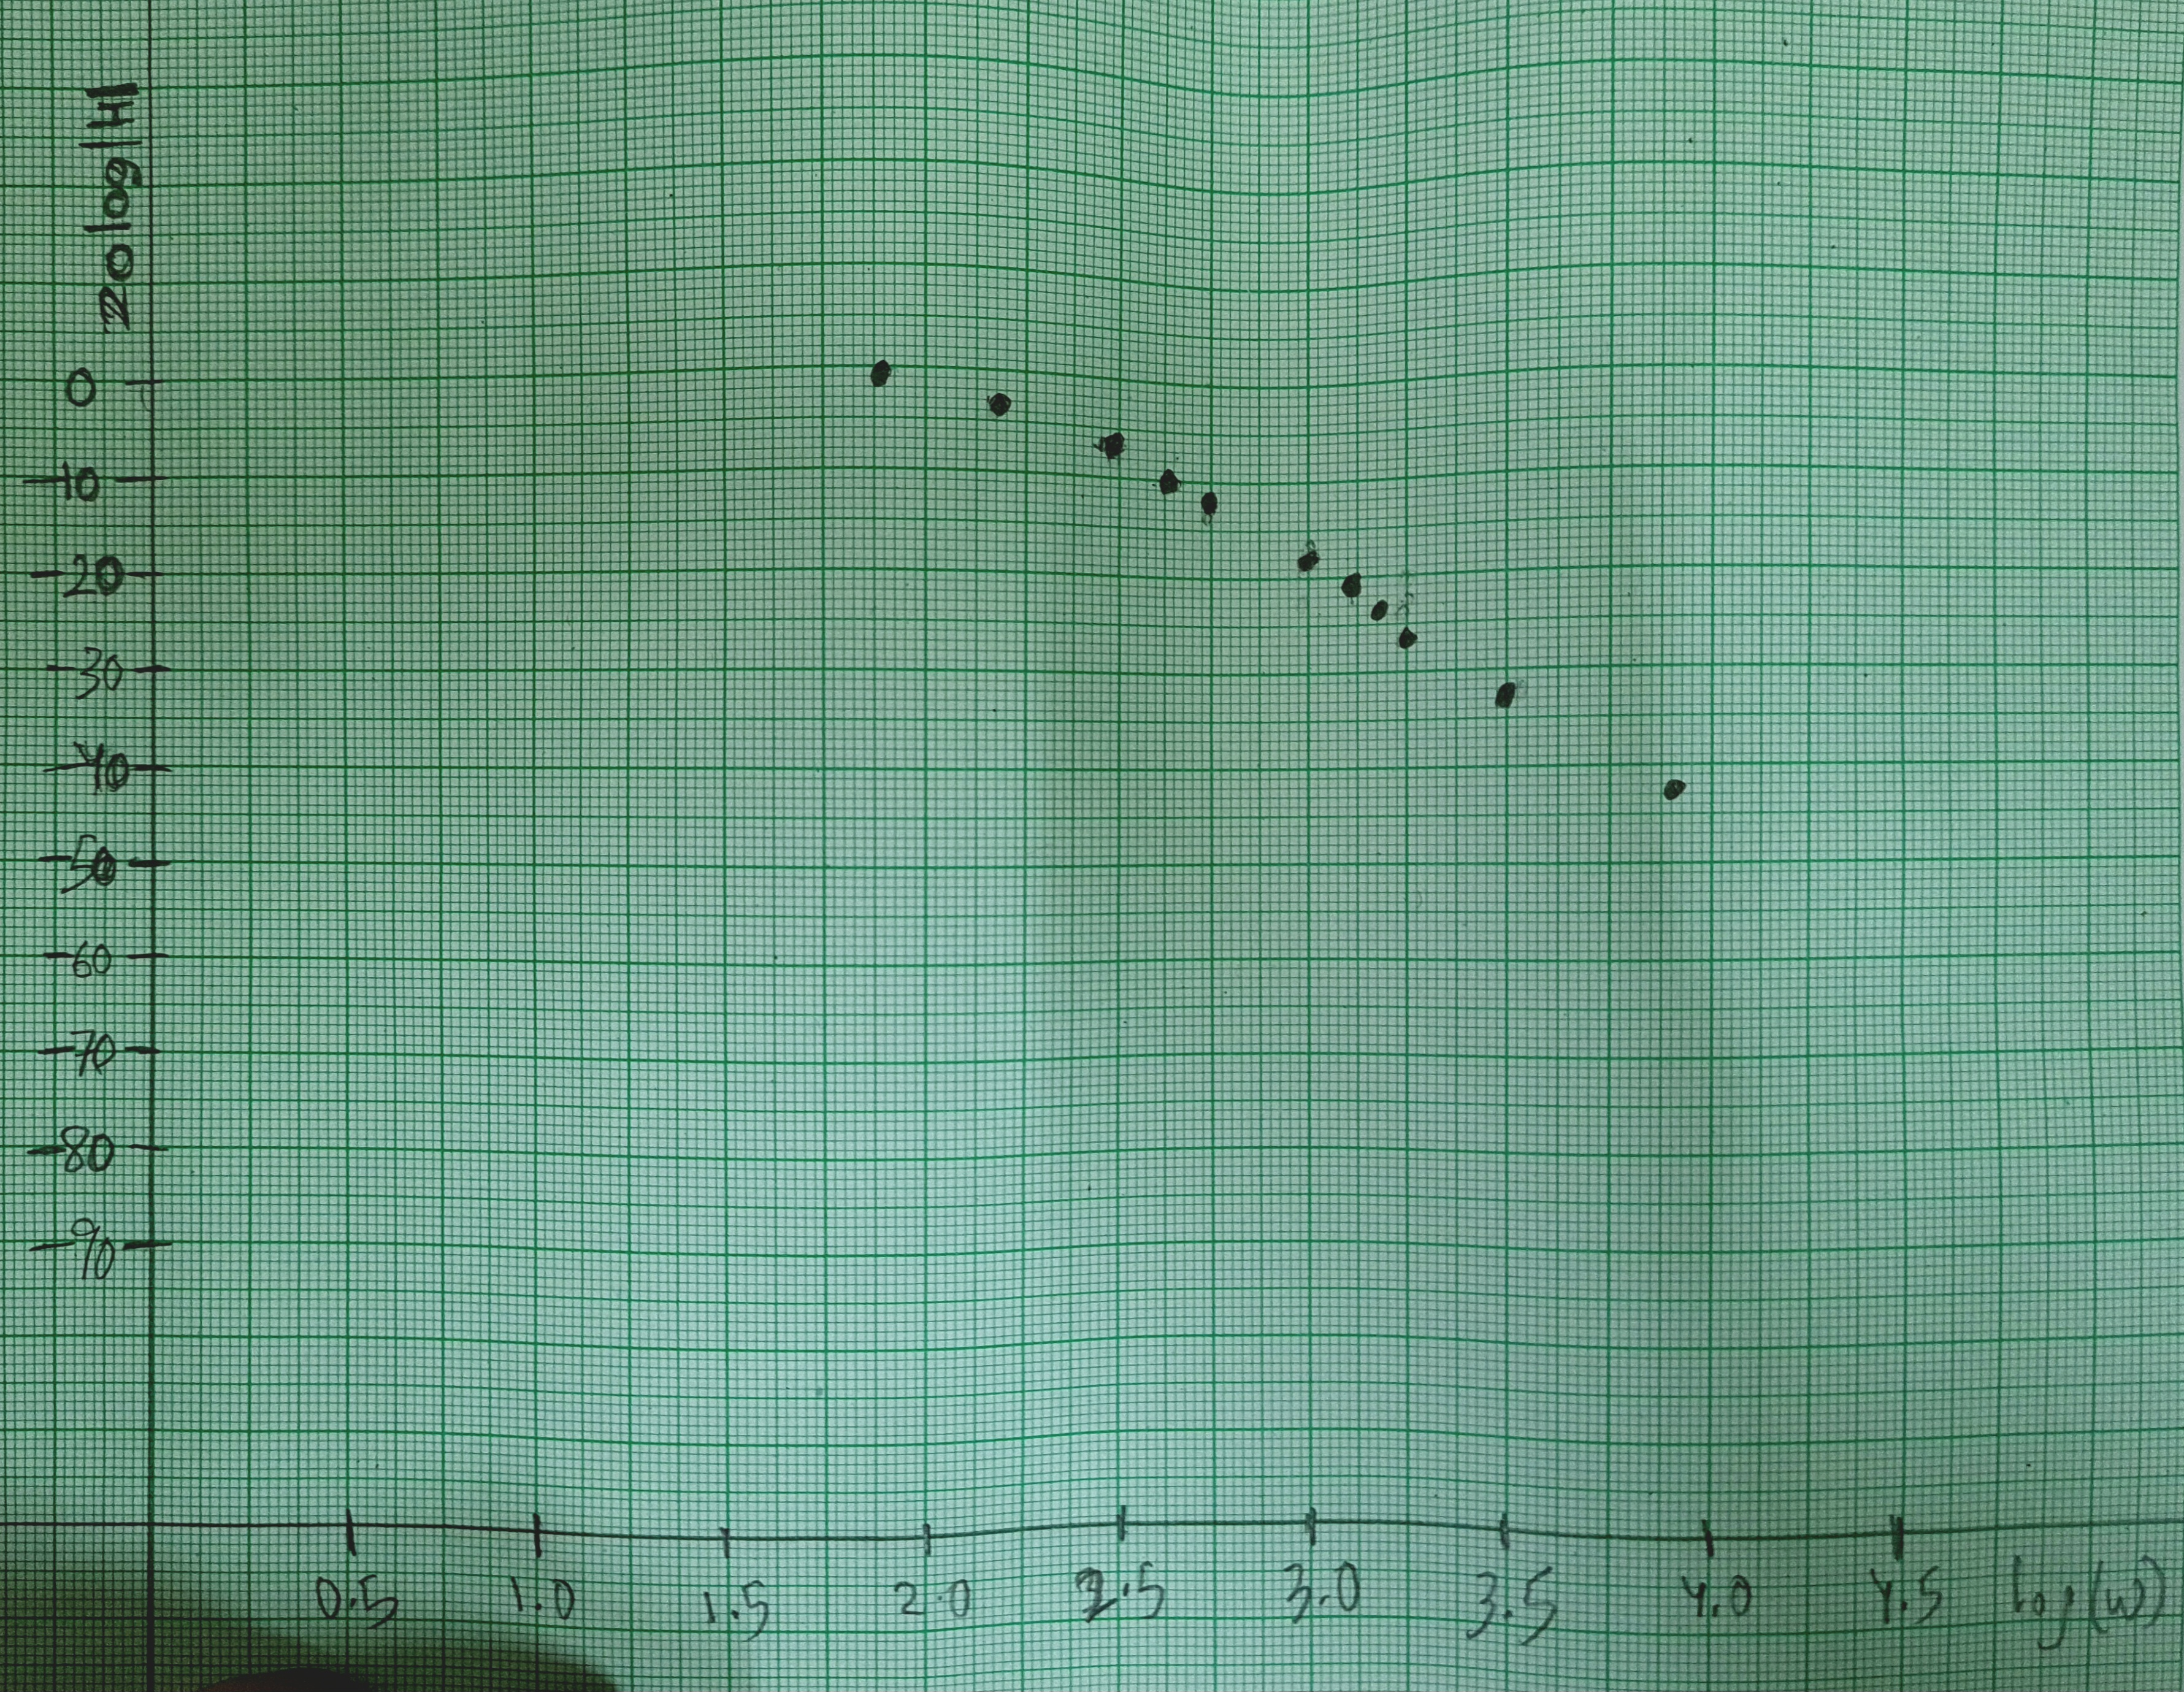
\includegraphics[width=0.7\columnwidth]{/home/gvt1/Work/ECLab2025/experiment03/files/GraphH2.jpg}
  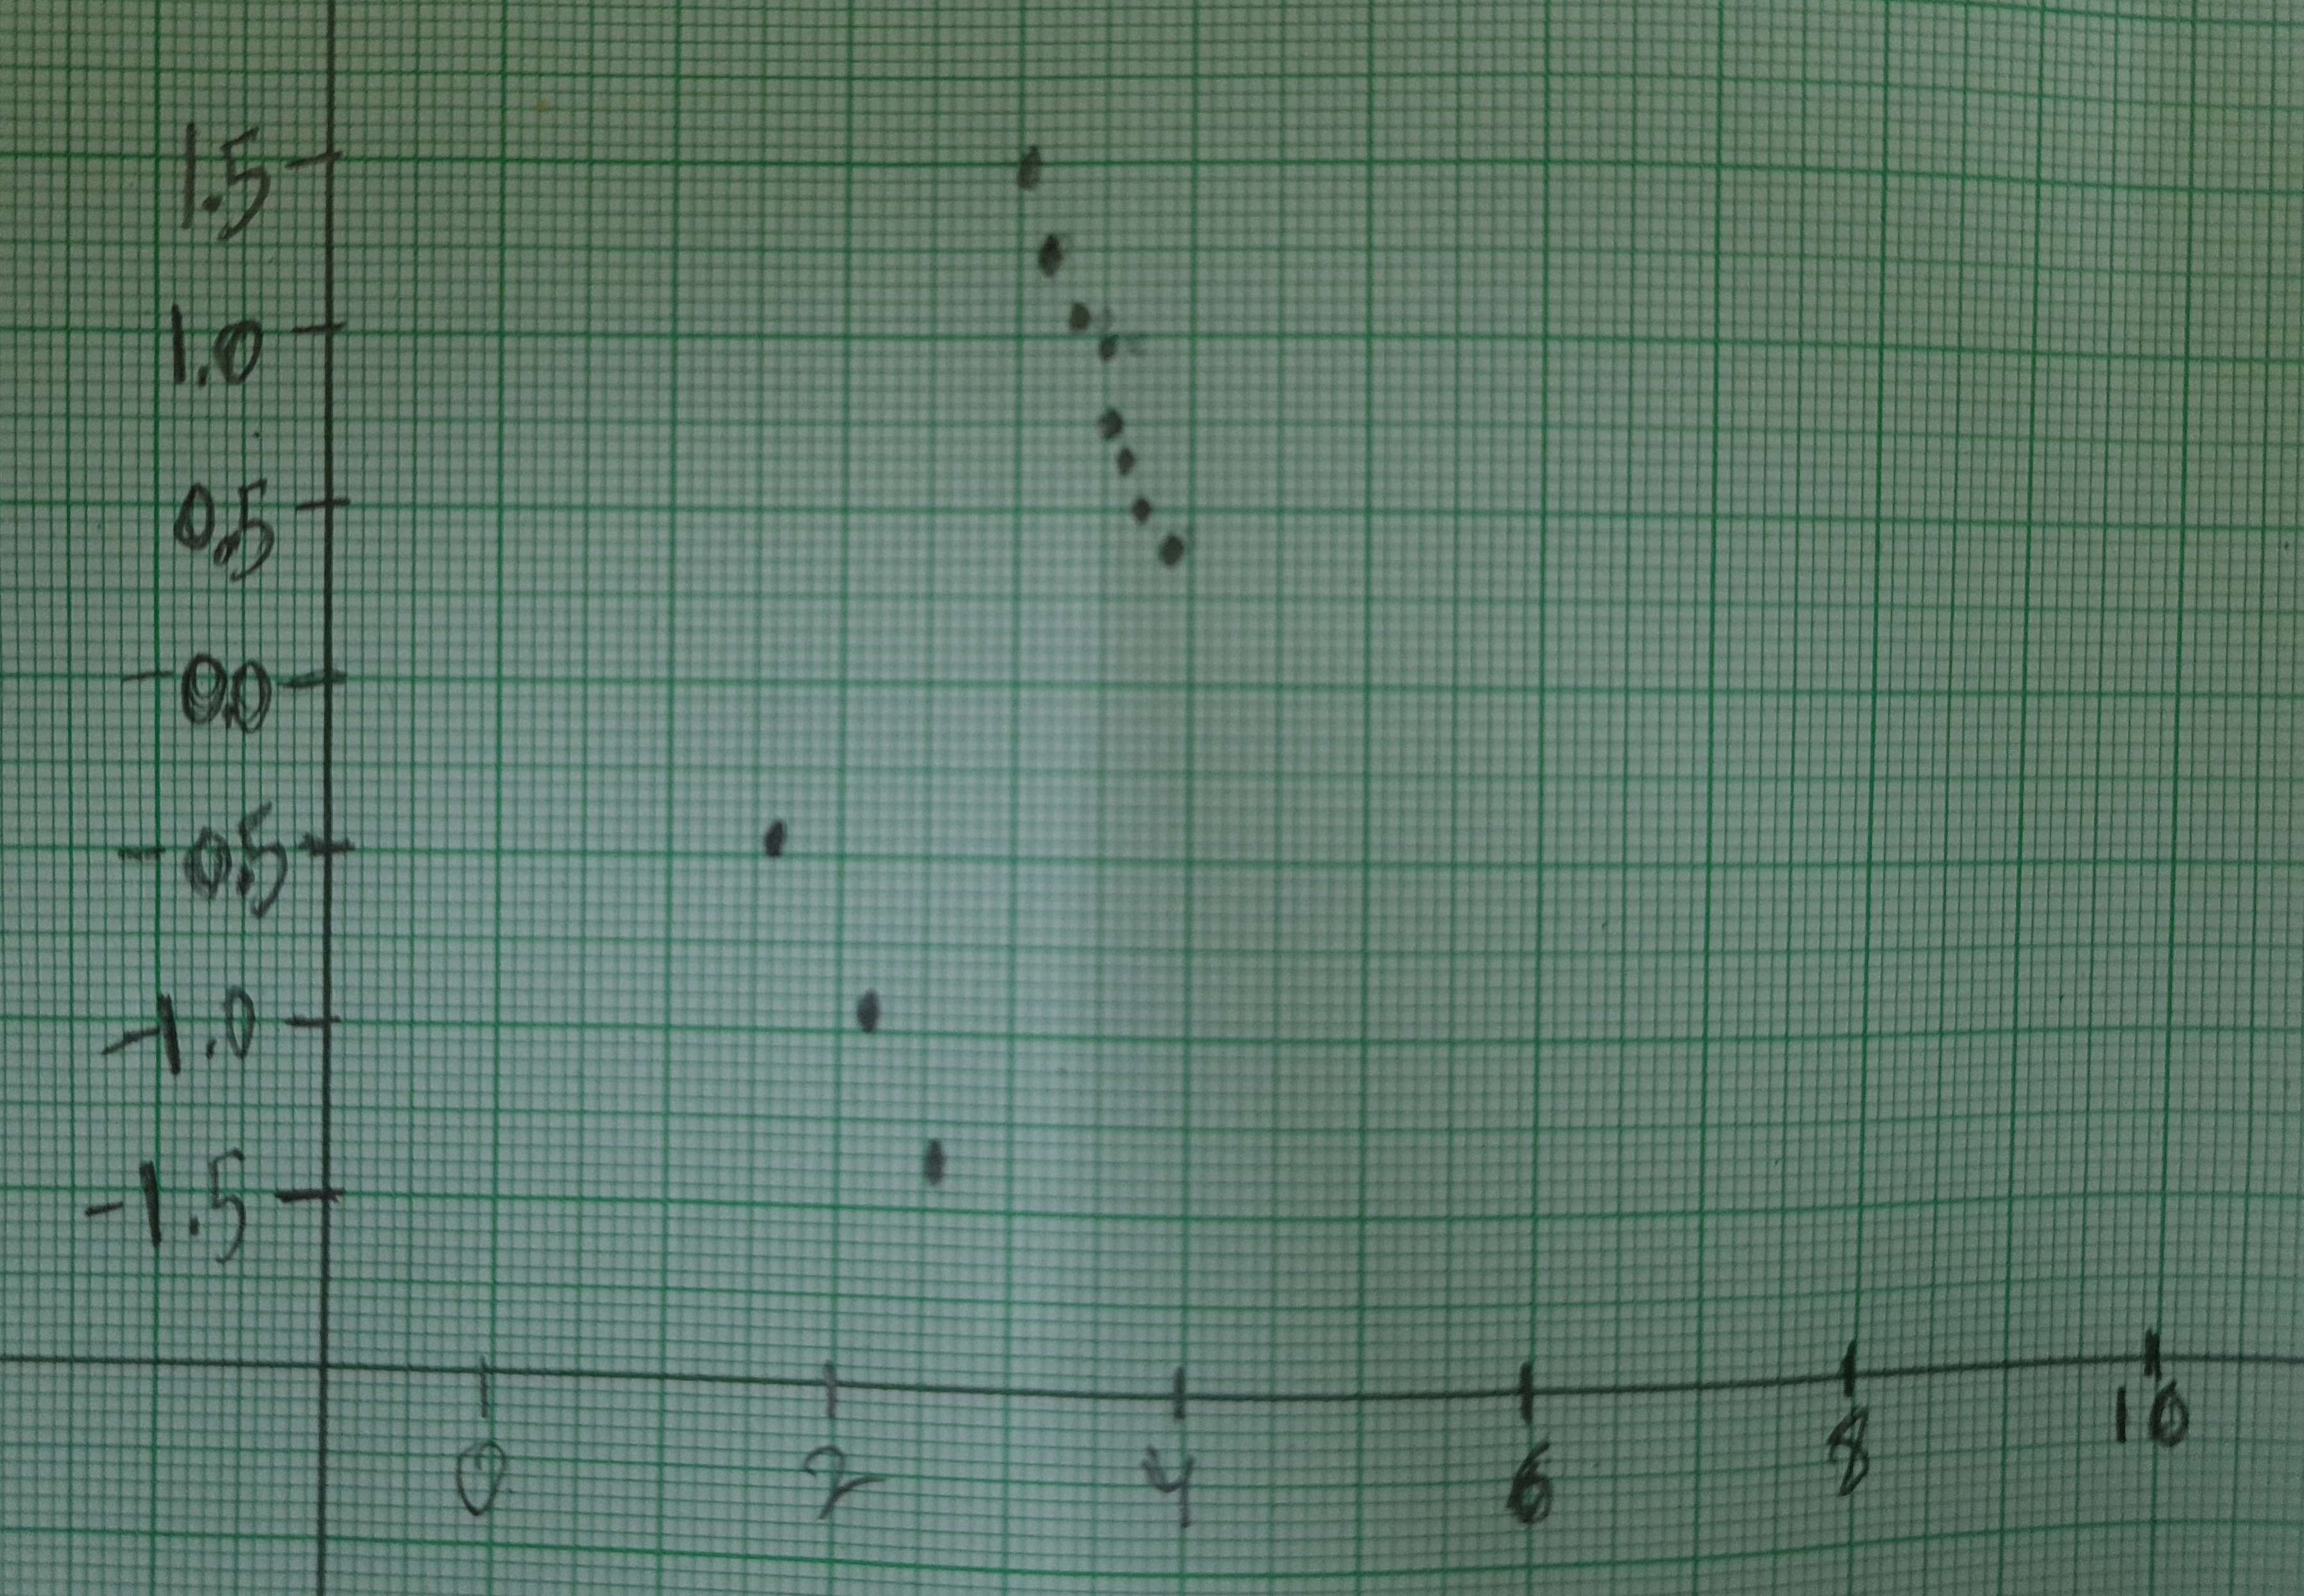
\includegraphics[width=0.4\columnwidth]{/home/gvt1/Work/ECLab2025/experiment03/files/GraphP2.jpg}
\end{figure}
\subsection{2-stage RC filter}
\begin{figure}[!ht]
\centering
  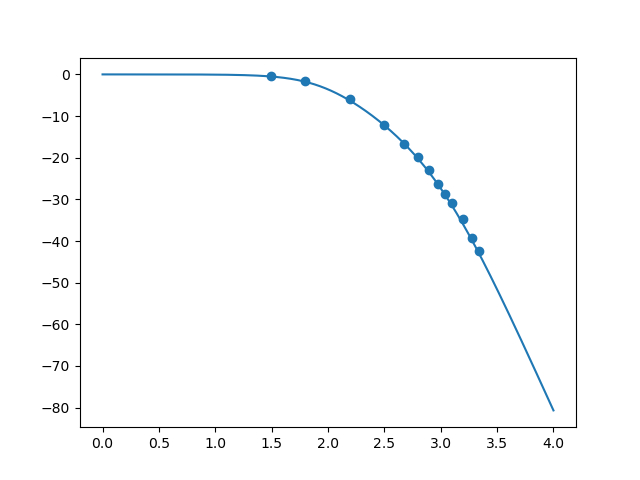
\includegraphics[width=0.4\columnwidth]{/home/gvt1/Work/ECLab2025/experiment03/files/fit_3.png}
  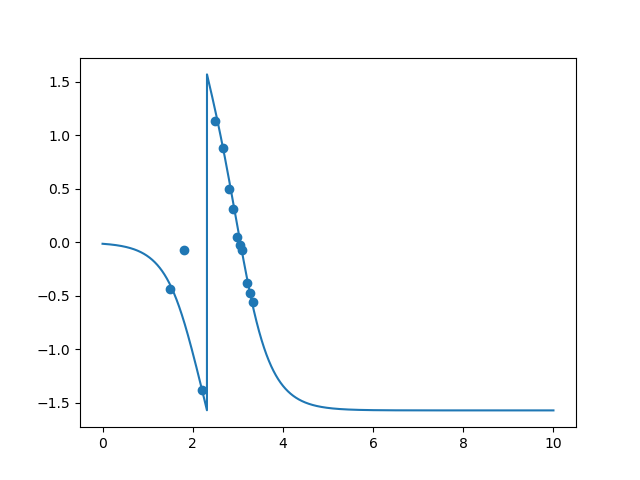
\includegraphics[width=0.4\columnwidth]{/home/gvt1/Work/ECLab2025/experiment03/files/phase_3.png}
  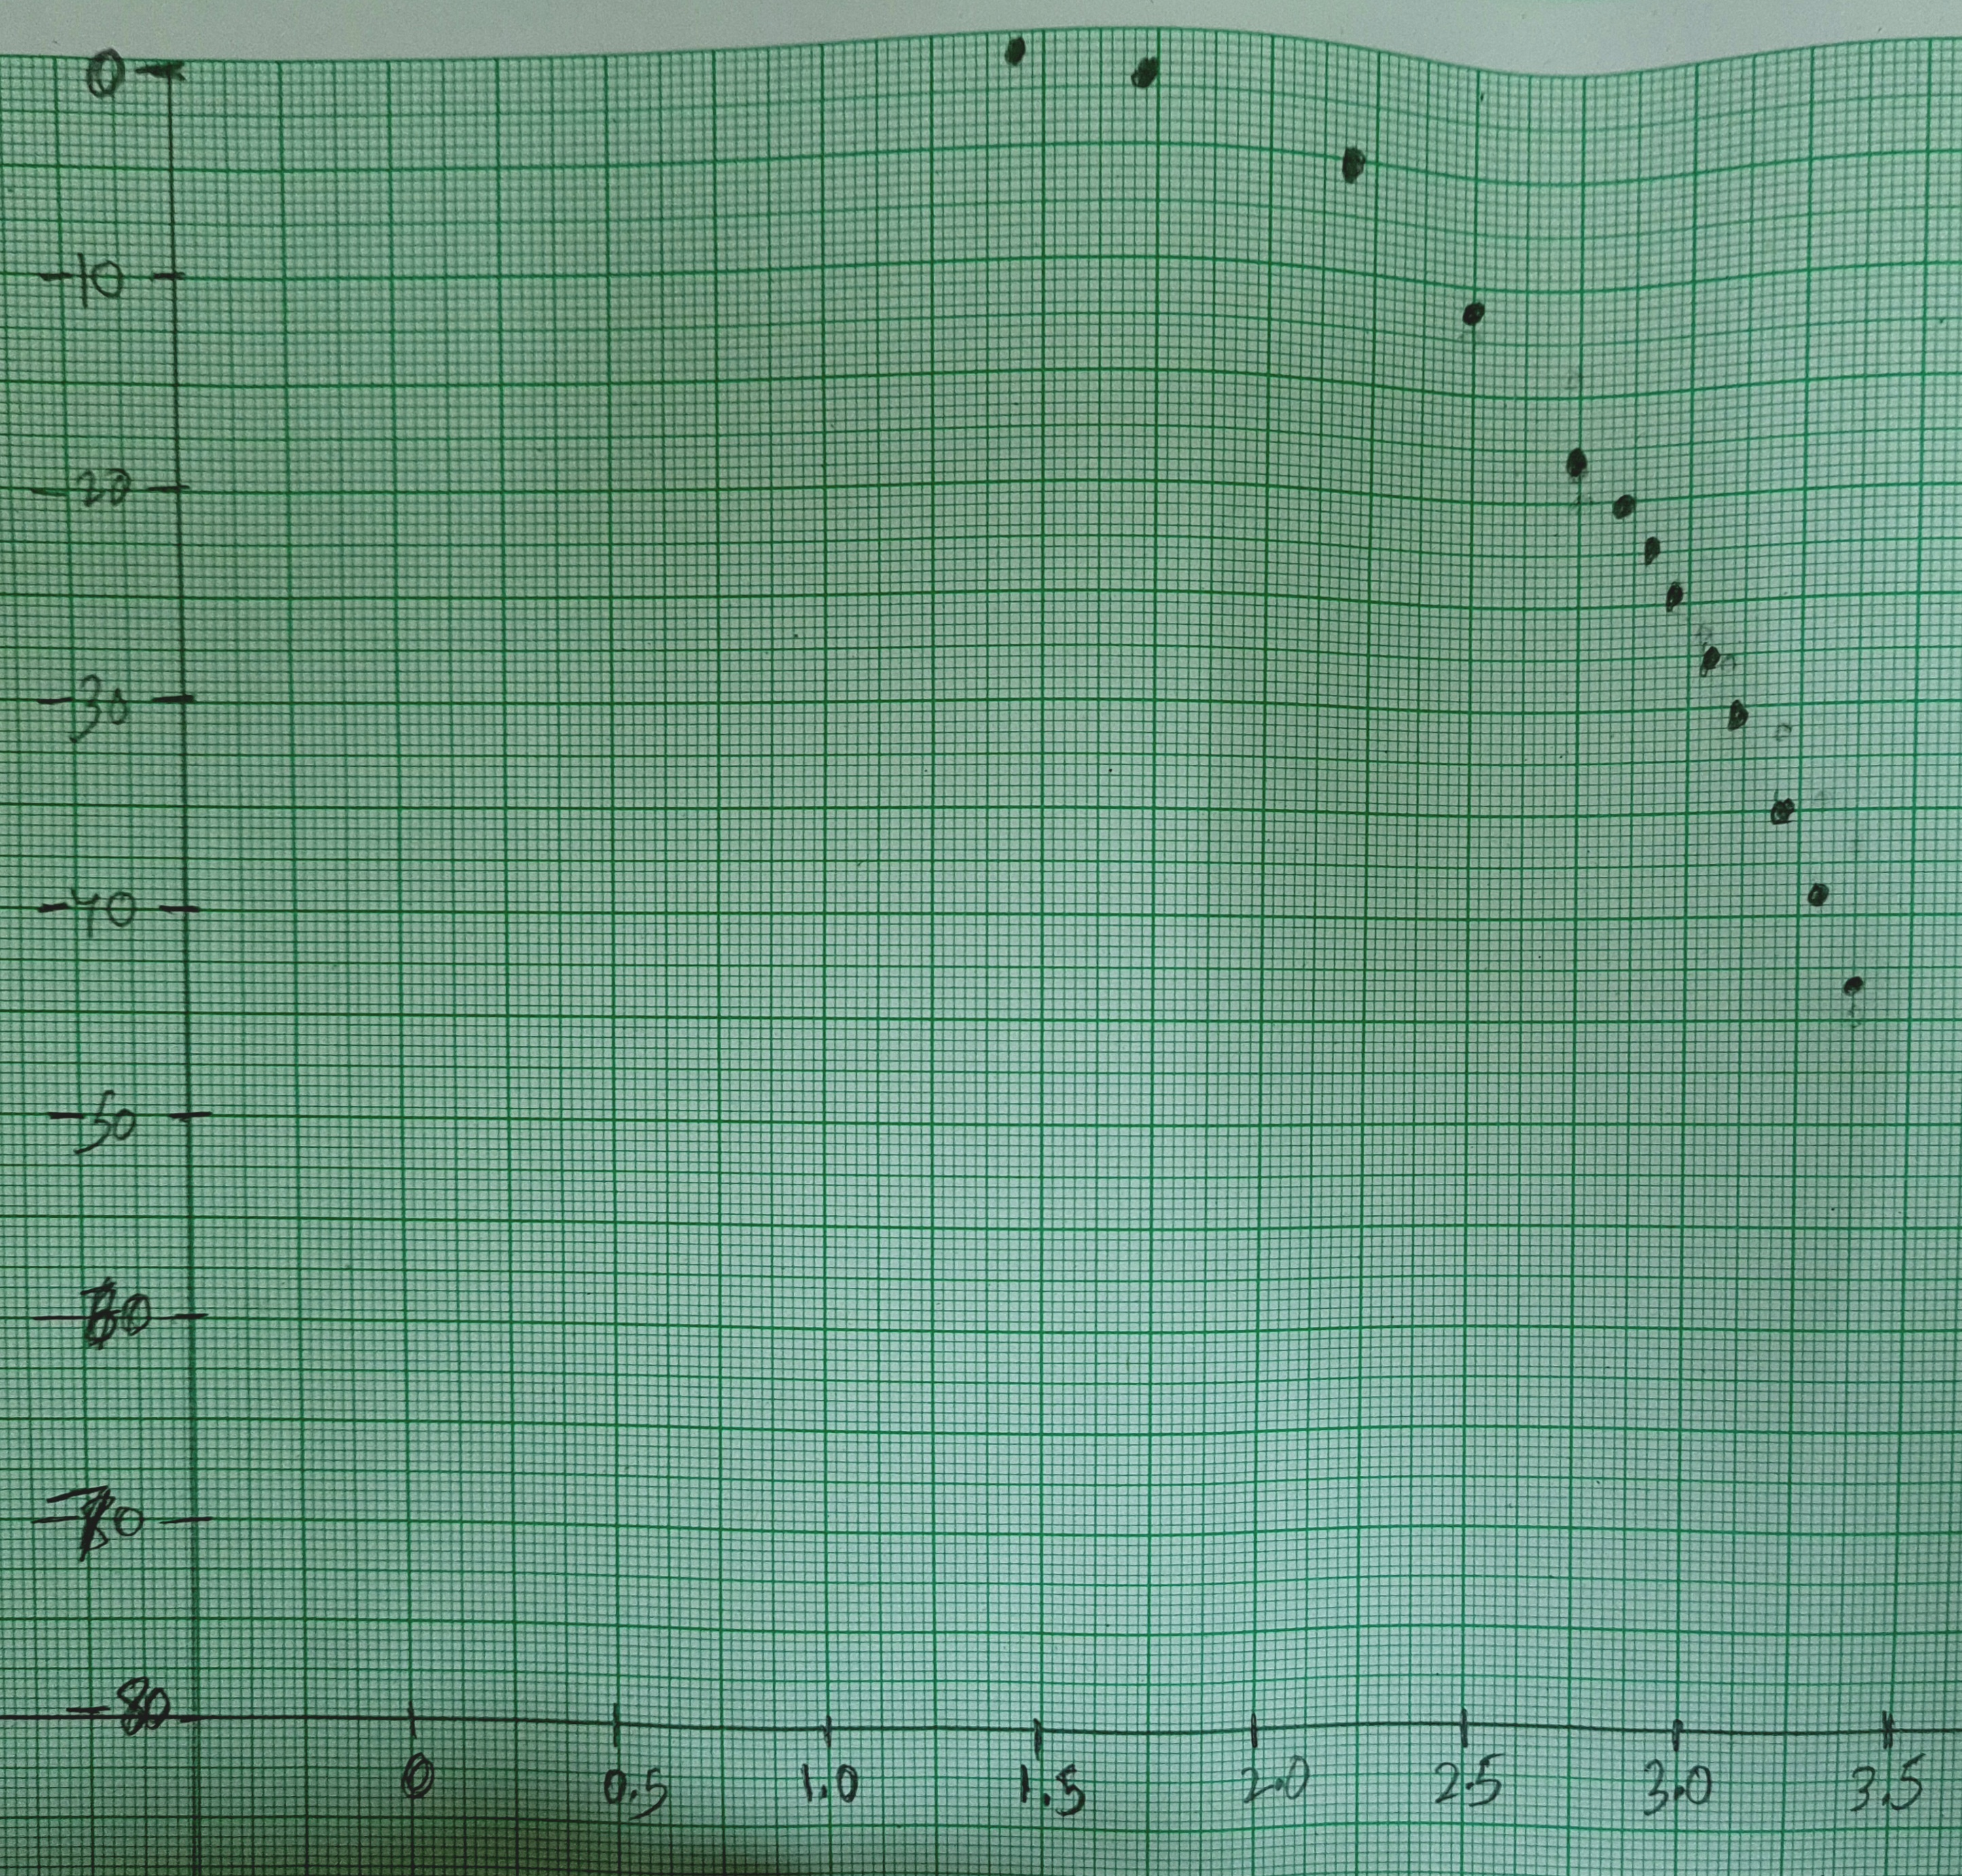
\includegraphics[width=0.7\columnwidth]{/home/gvt1/Work/ECLab2025/experiment03/files/GraphH3.jpg}
  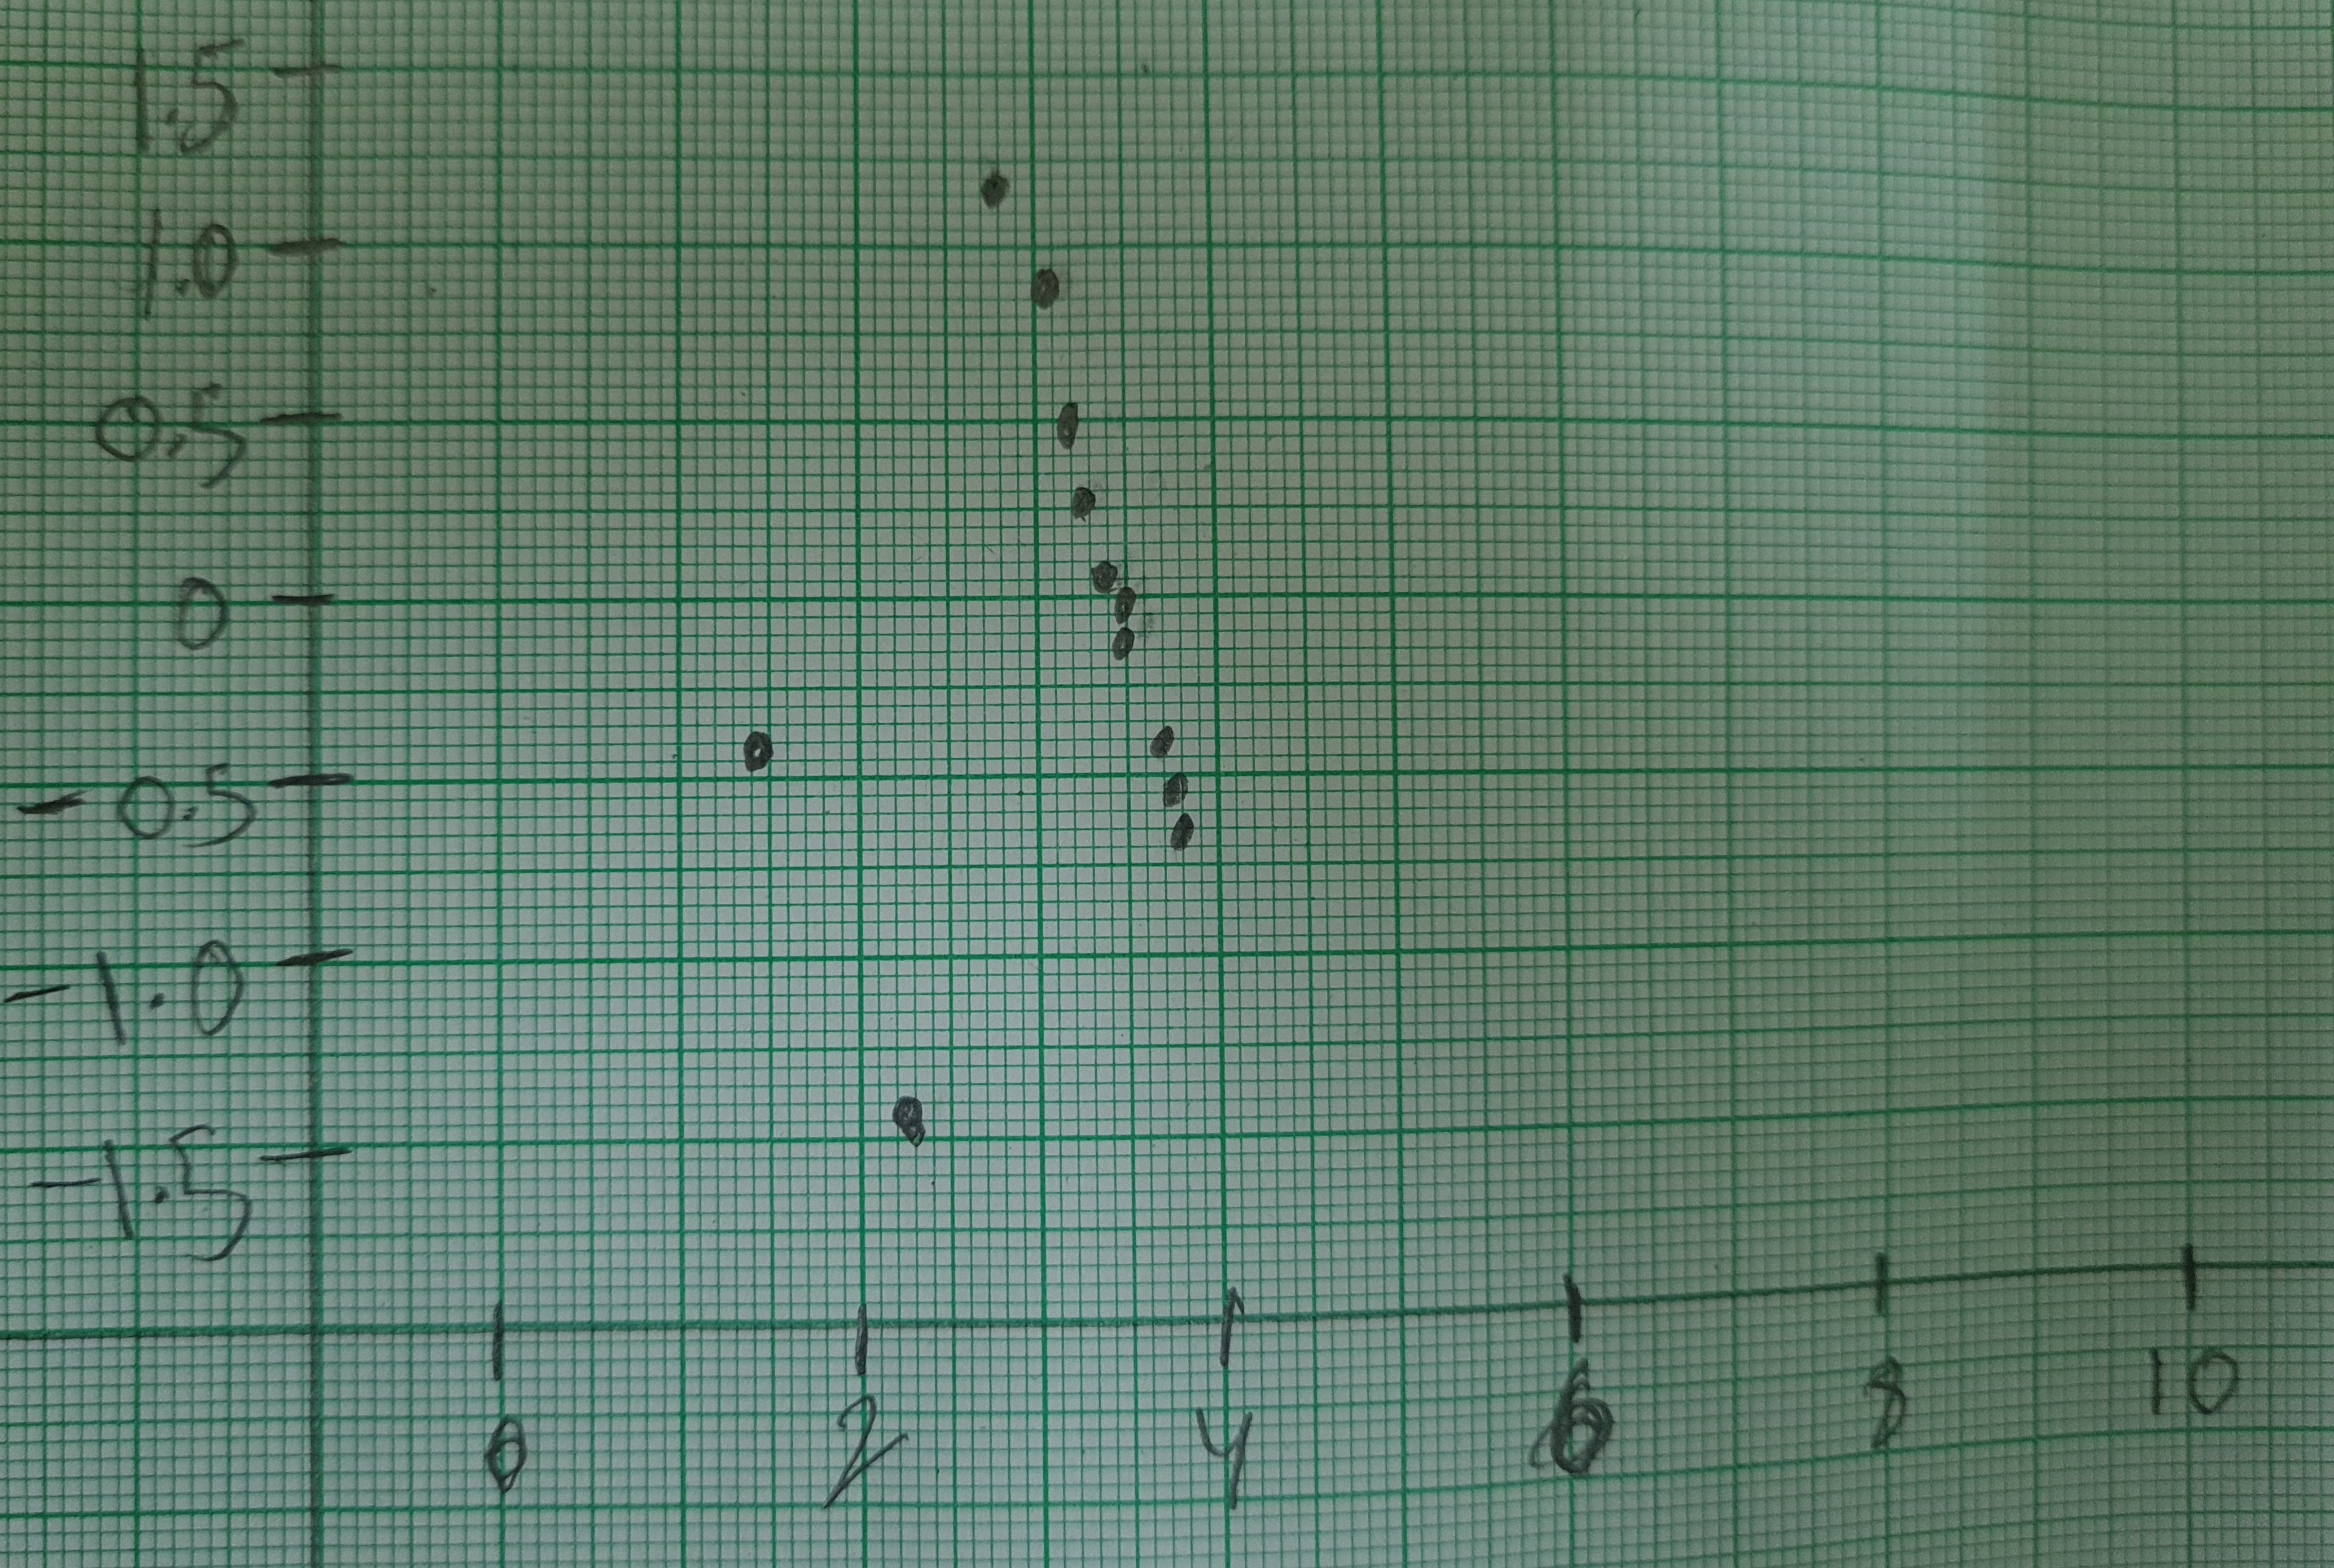
\includegraphics[width=0.4\columnwidth]{/home/gvt1/Work/ECLab2025/experiment03/files/GraphP3.jpg}
\end{figure}
\section{Conclusion}
In this experiment, we analyzed the frequency response of single-stage, two-stage, and three-stage RC low-pass filters. By measuring amplitude attenuation and phase shift across different frequencies, we observed that:  

\begin{itemize}  
    \item The magnitude response confirmed that increasing the number of cascaded RC stages resulted in a steeper roll-off, improving the filtering effect.  
    \item The phase response showed an increasing phase shift with higher frequencies, consistent with theoretical expectations.  
    \item The experimental data closely matched the theoretical transfer functions derived for each stage, with minor deviations likely due to component tolerances and measurement inaccuracies.  
    \item The frequency response plots demonstrated that higher-order filters provide better attenuation of high-frequency signals, making them more effective in signal conditioning applications.  
\end{itemize}  

Overall, this experiment provided hands-on validation of fundamental circuit analysis concepts and reinforced the importance of transfer function derivation in understanding filter behavior.
\end{document}

